\chapter{Análisis de software}

Hasta el momento conocemos la metodología utilizada para la investigación completa; sin embargo, es necesario especificar el desarrollo del software, ya que es necesario garantizar el correcto diseño e implementación del simulador para poder realizar las pruebas adecuadas con el menor número de errores. Es por esto que en este capítulo se detalla el proceso de desarrollo del simulador, lo que incluye la especificación de la metodología utilizada, requerimientos del sistema y modelado, diseño e implementación de cada una de las entregas.

\section{Metodología de desarrollo}

Para el desarrollo de software se utiliza un modelo de entrega por etapas. Este modelo, como se observa en la figura \ref{fig:modelo_etapas}, realiza las primeras etapas de forma secuencial y permite diseñar e implementar los componentes del proyecto por separado. Seguir este modelo permite entregar partes del proyecto y tener visibilidad del progreso. 

\begin{figure}[htbp]
	\centering
	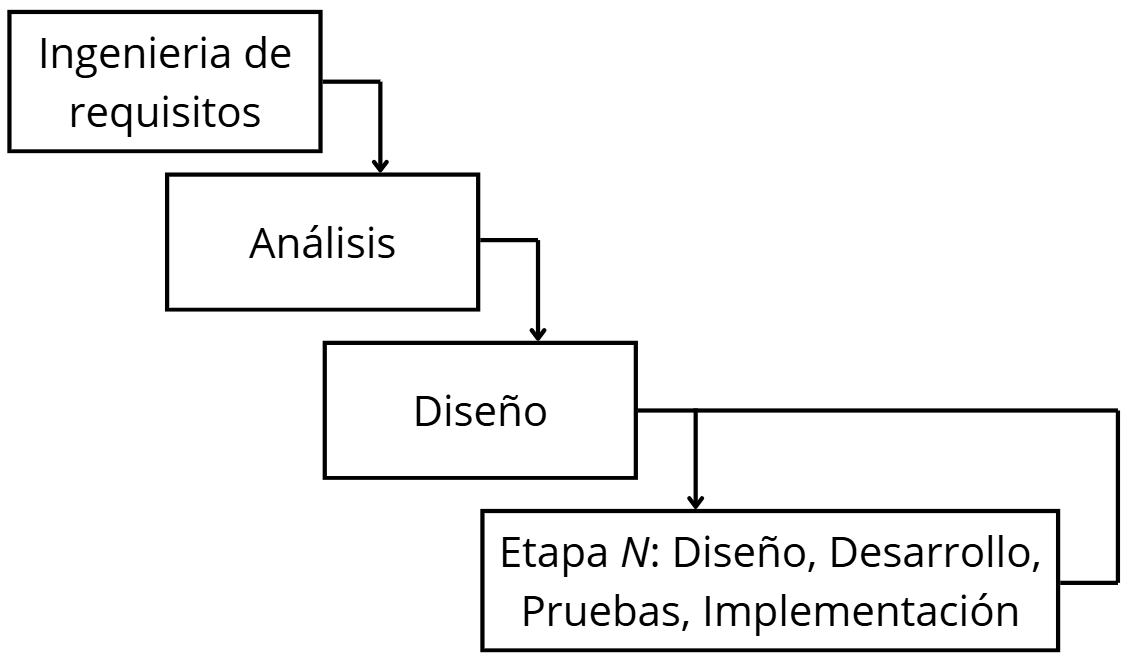
\includegraphics[width=0.75\linewidth]{img/modelo_etapas.png}
	\caption{Representación gráfica del modelo de entrega por etapas para el desarrollo del software}
	\label{fig:modelo_etapas}
\end{figure}

Estas son algunas de las razones por las cuales se opta por este modelo:

\begin{itemize}
	\item El tamaño del equipo de desarrollo es reducido: Al tener un número de integrantes reducido, resulta inviable desarrollar múltiples componentes de forma paralela. 
	
	\item No existe un cliente: El desarrollo de este producto de software es únicamente un medio para el proceso experimental.
	
	\item No es un producto comercial: No se planea monetizar dado que no existe un cliente. Por lo que en la ingeniería de requisitos se consideran los necesarios propuestos por el equipo de investigación para satisfacer las necesidades tecnológicas.
	
	\item No hay procesos iterativos: Al no tener cliente, no es necesario tener una validación externa, ni cambios significativos en los requerimientos del software. 
\end{itemize}

\begin{itemize}
	\item Simulador funcional de cualquier autómata celular en dos dimensiones en un espacio celular finito.
	
	\item Personalización de la vecindad, conjunto de estados, condición de frontera y función de transición.
	
	\item Personalización del diseño de estados e interacción en tiempo real con el espacio celular.
	
	\item Controles de simulación para avanzar, retroceder, reiniciar y manipular la velocidad de la animación.
\end{itemize}

Para mayor detalle de esta primera etapa, más adelante se especifican los casos de uso.

\section{Reglas de negocio}

\begin{enumerate}[label*=RN\arabic*]
	
	\item El estado de una célula en el tiempo $t + 1$ depende únicamente de su estado actual y de los estados de sus vecinos.
	
	\item Para iniciar la simulación es necesario que el conjunto de estados, la topología de la vecindad, la condición de frontera y la función de transición hayan sido definidos.
	
	\item Cuando la simulación está en curso, no se puede cambiar el conjunto de estados, la topología de la vecindad ni la función de transición.
	
	\item El usuario puede manipular el estado de una célula y la condición de frontera en tiempo de ejecución.
	
	\item Los datos importados deben cumplir con el formato definido por el sistema para garantizar su correcta interpretación.
	
	\item Los datos exportados deben conservar el mismo formato que los datos importados.
	
	\item El usuario puede pausar, detener, reanudar o retroceder la simulación sin pérdida de información. 
	
	\item Solo se permite una simulación activa por sesión.
	
\end{enumerate}

\section{Requerimientos}

\subsection{Requerimientos funcionales}

Los requerimientos funcionales describen las capacidades que el sistema debe ofrecer al usuario para cumplir con los objetivos establecidos.

\begin{enumerate}[label=RF\arabic*]
	
	\item El sistema debe mostrar una cuadrícula regular y finita que represente el espacio celular.
	
	\item El sistema debe permitir al usuario interactuar con el espacio celular, asignando o modificando los estados de las células.
	
	\item El sistema debe permitir al usuario definir el conjunto de estados, la topología de la vecindad local y las condiciones de frontera del espacio celular.
	
	\item El sistema debe permitir la evolución del espacio celular mediante un único paso o de forma continua, ajustando la velocidad de actualización según las capacidades computacionales del sistema.
	
	\item El sistema debe permitir la importación y exportación de configuraciones y evoluciones del espacio celular.
	
	\item El sistema debe permitir al usuario establecer la función de transición de manera manual.
	
	\item El sistema debe permitir configurar la red neuronal para imitar el comportamiento de una evolución señalada.
	
	\item El sistema debe entrenar una red neuronal dados los parámetros del usuario y la evolución que desea replicar.
	
\end{enumerate}

\subsection{Requerimientos no funcionales}

Los requerimientos no funcionales especifican las condiciones de calidad, desempeño y compatibilidad bajo las cuales el sistema debe operar.

\begin{enumerate}[label=RNF\arabic*.]
	
	\item El sistema debe poder ejecutarse en Fedora 42 sin requerir modificaciones en el código fuente.
	
	\item El sistema debe ser capaz de procesar al menos 10,000 células o registros por segundo utilizando una GPU NVIDIA RTX 5080.
	
	\item El sistema debe garantizar disponibilidad continua durante la ejecución, sin fallos o interrupciones críticas.
	
	\item La interfaz del sistema debe tener mensajes claros y funcionalidades bien definidas.
	
\end{enumerate}

\subsection{Requerimientos de sistema}

\subsubsection{Recomendado}

Los siguientes requerimientos describen el entorno principal y recomendado de ejecución, en el cual el sistema garantiza un rendimiento óptimo y estabilidad durante los procesos de simulación:

\begin{itemize}
	
	\item \textbf{Procesador:} Intel Core i9-14900K × 32 núcleos.
	
	\item \textbf{GPU:} NVIDIA GeForce RTX 5080.
	
	\item \textbf{Sistema operativo:} Fedora Linux 42 (Workstation Edition).
	
	\item \textbf{Entorno de escritorio:} GNOME 48.
	
	\item \textbf{Sistema de ventaneo:} Wayland.
	
\end{itemize}

\subsubsection{Mínimo}

También se establecen los requisitos mínimos necesarios para usar el simulador, teniendo en cuenta que el rendimiento y la velocidad de procesamiento dependerán de las capacidades del hardware disponible y que el entrenamiento podría no ser posible.

\begin{itemize}
	
	\item \textbf{Procesador:} Intel Core i7-1185G7 × 4 núcleos.
	
	\item \textbf{GPU:} Intel Corporation Raptor Lake-S GT1 [UHD Graphics 770].
	
	\item \textbf{Sistema operativo:} Fedora Linux 42 (Workstation Edition).
	
	\item \textbf{Entorno de escritorio:} GNOME 48.
	
	\item \textbf{Sistema de ventaneo:} Wayland.
	
\end{itemize}